\documentclass[tikz,border=8pt]{standalone}
\usetikzlibrary{arrows.meta,positioning,fit}
\begin{document}
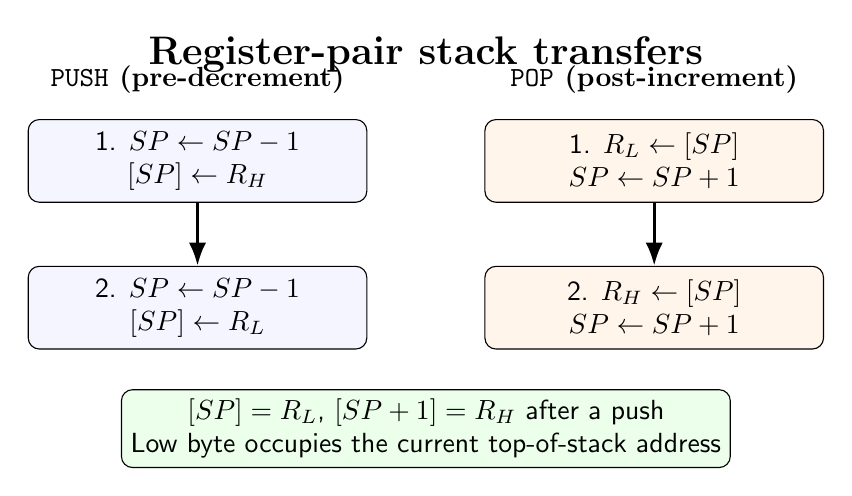
\begin{tikzpicture}[font=\sffamily,>=Latex,opbox/.style={draw,rounded corners,minimum width=4.3cm,minimum height=1.05cm,align=center,fill=blue!4},popbox/.style={opbox,fill=orange!8}]
\node[font=\Large\bfseries] at (5.4,5.0) {Register-pair stack transfers};
\node[opbox] (p1) at (2.5,3.65) {1. $SP\leftarrow SP-1$\\$[SP]\leftarrow R_H$};
\node[opbox,below=8mm of p1] (p2) {2. $SP\leftarrow SP-1$\\$[SP]\leftarrow R_L$};
\node[above=2mm of p1,font=\bfseries] {\texttt{PUSH} (pre-decrement)};
\node[popbox] (q1) at (8.3,3.65) {1. $R_L\leftarrow[SP]$\\$SP\leftarrow SP+1$};
\node[popbox,below=8mm of q1] (q2) {2. $R_H\leftarrow[SP]$\\$SP\leftarrow SP+1$};
\node[above=2mm of q1,font=\bfseries] {\texttt{POP} (post-increment)};
\draw[very thick,->] (p1)--(p2);
\draw[very thick,->] (q1)--(q2);
\node[draw,rounded corners,fill=green!8,align=center] at (5.4,.25) {$[SP]=R_L$, $[SP+1]=R_H$ after a push\\Low byte occupies the current top-of-stack address};
\end{tikzpicture}
\end{document}
